\documentclass[10pt,a4paper]{article}
\usepackage[utf8]{inputenc}
\usepackage[T1]{fontenc}
\usepackage{lmodern}
\usepackage[english]{babel}
\usepackage[margin=2.0cm]{geometry}
\usepackage{amsmath,amssymb,mathtools,bm}
\usepackage{booktabs,array,tabularx,longtable}
\newcolumntype{L}[1]{>{\raggedright\arraybackslash}p{#1}}
\newcolumntype{Y}{>{\raggedright\arraybackslash}X}
\usepackage{graphicx}
\usepackage{float}
\usepackage[font=small]{caption}
\usepackage{xcolor}
\usepackage{tikz}
\usetikzlibrary{arrows.meta,positioning,decorations.pathmorphing,decorations.pathreplacing,patterns,calc}
\usepackage[hidelinks]{hyperref}
\usepackage{url}
\makeatletter\g@addto@macro{\UrlBreaks}{\do\_\do/}\makeatother
\numberwithin{equation}{section}
\setlength{\emergencystretch}{3em}
\newcommand{\note}[1]{\begin{center}\fcolorbox{red!70!black}{red!5}{\parbox{0.94\linewidth}{\small\textbf{Note.} #1}}\end{center}}
\newcommand{\costP}{0.000985}
\newcommand{\costA}{0.000273}
\newcommand{\nStartsP}{10}
\newcommand{\nStartsA}{8}
\newcommand{\nStartsPbest}{10}
\newcommand{\nStartsAbest}{8}
\newcommand{\costsA}{0.000273}
\newcommand{\nBoundP}{10}
\newcommand{\nParP}{21}
\newcommand{\nBoundA}{9}
\newcommand{\nParA}{15}
\newcommand{\kg}{129}
\newcommand{\etag}{2.72}
\newcommand{\kgA}{1015}
\newcommand{\etaA}{0.51}
\newcommand{\taudA}{0.48}
\newcommand{\alphaA}{0.625}
\newcommand{\kLA}{\ensuremath{5.61\times10^{4}}}
\newcommand{\Kt}{0.258}
\newcommand{\fCL}{1.5}
\newcommand{\JL}{0.588}
\newcommand{\JAP}{2.008}
\newcommand{\kgPrev}{117}
\newcommand{\etagPrev}{3.20}
\newcommand{\fMassI}{56.7}
\newcommand{\aMassI}{$-$0.566}
\newcommand{\JMassI}{1.77}
\newcommand{\zMassI}{0.033}
\newcommand{\zStdI}{6.9\,\%}
\newcommand{\aLogI}{$-$0.695}
\newcommand{\zLogI}{0.038}
\newcommand{\aStepI}{$-$0.270}
\newcommand{\fStepI}{56.4}
\newcommand{\fMassII}{99.0}
\newcommand{\aMassII}{+0.650}
\newcommand{\JMassII}{1.54}
\newcommand{\zMassII}{0.033}
\newcommand{\zStdII}{10.3\,\%}
\newcommand{\aLogII}{+0.626}
\newcommand{\zLogII}{0.030}
\newcommand{\aStepII}{+0.303}
\newcommand{\fStepII}{98.7}
\newcommand{\fBearP}{1.76}
\newcommand{\etaBearP}{2.70}
\newcommand{\fShaftP}{316}
\newcommand{\fShaftPb}{815}
\newcommand{\fBearA}{3.13}
\newcommand{\etaBearA}{0.51}
\newcommand{\fForkA}{56.2}
\newcommand{\etaForkA}{0.0055}
\newcommand{\fShaftA}{948}
\newcommand{\zForkA}{0.028}
\newcommand{\zForkStd}{6.2\,\%}
\newcommand{\zForkStep}{0.010}
\newcommand{\fForkStep}{56.6}
\newcommand{\kgStep}{122}
\newcommand{\etagStep}{2.86}
\newcommand{\kgAStep}{955}
\newcommand{\etaAStep}{0.62}
\newcommand{\alphaStep}{0.428}
\newcommand{\kLAStep}{\ensuremath{7.06\times10^{4}}}
\newcommand{\costPStep}{0.0012}
\newcommand{\costAStep}{0.000929}
\newcommand{\zetaMax}{0.05}
\newcommand{\zetaMaxStep}{0.01}
\newcommand{\cadJ}{20}
\newcommand{\cadK}{20}
\newcommand{\sJLA}{1.20}
\newcommand{\sJhpP}{1.177}
\newcommand{\sJLAStepJ}{1.15}
\newcommand{\costPStepJ}{0.000985}
\newcommand{\costAStepJ}{0.000727}
\newcommand{\costRedA}{23}
\newcommand{\costRedKt}{51}
\newcommand{\costRedKtP}{0.000}
\newcommand{\gKtA}{0.90}
\newcommand{\gKtP}{1.007}
\newcommand{\KtA}{0.232}
\newcommand{\ktVar}{10}
\newcommand{\ktLo}{0.90}
\newcommand{\ktHi}{1.10}
\newcommand{\sktwoAFour}{1.20}
\newcommand{\sJLAFour}{1.20}
\newcommand{\JtotAFour}{2.596}
\newcommand{\costRedAInter}{1.8}
\newcommand{\fitAInter}{59}
\newcommand{\sktwoA}{1.20}
\newcommand{\costRedP}{0.08}
\newcommand{\JtotA}{2.596}
\newcommand{\JtotAStepJ}{2.488}
\newcommand{\cadCostP}{0.1}
\newcommand{\cadCostA}{2.5}
\newcommand{\nmpDisc}{\ensuremath{-6.9\times10^{10}}}
\newcommand{\nmpF}{73.4}
\newcommand{\nmpZeta}{0.318}
\newcommand{\nmpDiscStep}{\ensuremath{-4\times10^{9}}}
\newcommand{\nmpFStep}{74.0}
\newcommand{\nmpZetaStep}{0.073}
\newcommand{\Jaxis}{1.059}
\newcommand{\fitPI}{60}
\newcommand{\dbPI}{2.7}
\newcommand{\degPI}{18.4}
\newcommand{\fitLowPI}{66.9}
\newcommand{\fitPII}{69}
\newcommand{\dbPII}{2.4}
\newcommand{\degPII}{11.2}
\newcommand{\fitLowPII}{--}
\newcommand{\fitPIII}{65}
\newcommand{\dbPIII}{2.1}
\newcommand{\degPIII}{8.5}
\newcommand{\fitLowPIII}{--}
\newcommand{\fitA}{75}
\newcommand{\dbA}{2.5}
\newcommand{\degA}{17.2}
\newcommand{\fitLowA}{89.2}
\newcommand{\fitPIStep}{58}
\newcommand{\dbPIStep}{7.0}
\newcommand{\degPIStep}{20.0}
\newcommand{\fitLowPIStep}{66.2}
\newcommand{\fitPIIStep}{43}
\newcommand{\dbPIIStep}{11.7}
\newcommand{\degPIIStep}{18.2}
\newcommand{\fitLowPIIStep}{--}
\newcommand{\fitPIIIStep}{46}
\newcommand{\dbPIIIStep}{11.8}
\newcommand{\degPIIIStep}{16.1}
\newcommand{\fitLowPIIIStep}{--}
\newcommand{\fitAStep}{54}
\newcommand{\dbAStep}{2.6}
\newcommand{\degAStep}{15.6}
\newcommand{\fitLowAStep}{80.3}
\newcommand{\fitPIStepJ}{60}
\newcommand{\dbPIStepJ}{2.7}
\newcommand{\degPIStepJ}{18.4}
\newcommand{\fitLowPIStepJ}{66.6}
\newcommand{\fitPIIStepJ}{69}
\newcommand{\dbPIIStepJ}{2.4}
\newcommand{\degPIIStepJ}{11.2}
\newcommand{\fitLowPIIStepJ}{--}
\newcommand{\fitPIIIStepJ}{65}
\newcommand{\dbPIIIStepJ}{2.1}
\newcommand{\degPIIIStepJ}{8.6}
\newcommand{\fitLowPIIIStepJ}{--}
\newcommand{\fitAStepJ}{59}
\newcommand{\dbAStepJ}{3.0}
\newcommand{\degAStepJ}{17.2}
\newcommand{\fitLowAStepJ}{80.9}
\newcommand{\fitPIFour}{60}
\newcommand{\dbPIFour}{2.7}
\newcommand{\degPIFour}{18.4}
\newcommand{\fitLowPIFour}{66.9}
\newcommand{\fitPIIFour}{69}
\newcommand{\dbPIIFour}{2.4}
\newcommand{\degPIIFour}{11.2}
\newcommand{\fitLowPIIFour}{--}
\newcommand{\fitPIIIFour}{65}
\newcommand{\dbPIIIFour}{2.1}
\newcommand{\degPIIIFour}{8.5}
\newcommand{\fitLowPIIIFour}{--}
\newcommand{\fitAFour}{64}
\newcommand{\dbAFour}{2.8}
\newcommand{\degAFour}{17.2}
\newcommand{\fitLowAFour}{83.7}
\newcommand{\fitPICad}{60}
\newcommand{\dbPICad}{2.7}
\newcommand{\degPICad}{18.4}
\newcommand{\fitLowPICad}{66.9}
\newcommand{\fitPIICad}{68}
\newcommand{\dbPIICad}{2.5}
\newcommand{\degPIICad}{11.2}
\newcommand{\fitLowPIICad}{--}
\newcommand{\fitPIIICad}{65}
\newcommand{\dbPIIICad}{2.0}
\newcommand{\degPIIICad}{8.6}
\newcommand{\fitLowPIIICad}{--}
\newcommand{\fitACad}{84}
\newcommand{\dbACad}{1.6}
\newcommand{\degACad}{12.8}
\newcommand{\fitLowACad}{90.6}
\newcommand{\boundP}{$s_{J_e}$, $s_{J_m}$, $s_{J_\mathrm{rear}}$, $s_{k_{\theta1}}$, $s_{k_{\theta2}}$, $s_{k_{\theta3}}$, $\zeta_1$, $\zeta_4$, $\zeta_5$, $\zeta_6$}
\newcommand{\boundA}{$s_{J_e}$, $s_{J_m}$, $s_{J_L}$, $s_{k_1}$, $s_{k_2}$, $g_{K_t}$, $\zeta_1$, $\zeta_3$, $\zeta_4$}


\tikzset{
  mass/.style={draw, thick, fill=gray!8, minimum width=1.45cm, minimum height=0.95cm, align=center, font=\small},
  spring/.style={decorate, decoration={zigzag, pre length=2.5mm, post length=2.5mm, segment length=5pt, amplitude=3pt}},
  lab/.style={font=\scriptsize, inner sep=1.5pt},
  sig/.style={-{Latex[length=2mm]}, thick},
  meas/.style={-{Latex[length=2mm]}, dashed, blue!60!black},
  blk/.style={draw, rounded corners, align=center, minimum height=0.9cm, fill=blue!4, font=\small},
}
\newcommand{\ground}[3]{\draw[thick] (#1,#3) -- (#2,#3); \fill[pattern=north east lines] (#1,#3) rectangle (#2,#3-0.18);}

\title{Modal least-squares identification of the fork modes of the LUCY mount:\\ elevation axis with two stator modal masses and azimuth axis with a flexible load}
\author{Generated by \texttt{build\_fork\_modes\_report.py}\\ \small\texttt{sim/gimbal\_multidof/report\_fork\_modes}}
\date{\today}
\begin{document}
\maketitle

\paragraph{Purpose.} The resonances of the LUCY mount below 150\,Hz are vibrations of the fork. On the elevation axis they are excited by the motor stator and read by the encoder, which is mounted on the same structure. A first step modelled them with two modal masses attached to the stator (elevation) and a fork split into base and top (azimuth), using a logarithmic error and a robust cost with free damping. A second step repeated the identification of both axes with a modal least-squares method and modal damping $\zeta_k\leq\zetaMaxStep$. That limit proved too tight for the fork modes. A third step raised it to $\zeta_k\leq\zetaMax$, starting from the second-step result. A fourth step widened the tolerances on the CAD inertias and stiffnesses from $\pm15$ to $\pm\cadJ$\,\%. This report presents the final identification (fifth step): as the fourth step, with the motor torque constant $K_t$ free within its catalogue tolerance of $\pm\ktVar$\,\%, one factor per axis. The methodology is:
\begin{itemize}
\item a \textbf{modal formulation}: every mode is written in modal coordinates, with its own viscous modal damping;
\item \textbf{least squares on the real and imaginary parts} of the frequency response: no logarithm, quadratic cost;
\item \textbf{constraints}:
  \begin{itemize}
  \item modal damping ratios $\zeta_k\leq\zetaMax$ (\zetaMaxStep\ in the second step);
  \item CAD inertias and stiffnesses within $\pm\cadJ$\,\% of their values ($\pm15$\,\% up to the third step);
  \item torque constant within the Kollmorgen catalogue tolerance: $g_{K_t}K_t$ with $g_{K_t}\in[\ktLo,\ktHi]$ for each axis;
  \item ground stiffnesses, stiffnesses introduced in the model, and the modal parameters of the two stator masses free;
  \end{itemize}
\item the \textbf{telescope rigidly attached to the ring};
\item the \textbf{bearings modelled as a linear hysteretic element}.
\end{itemize}
All the results refer to the fit band \textbf{1--150\,Hz}.

\paragraph{Main results.}
\begin{itemize}
\item \textbf{Convergence.} All \nStartsP\ elevation starts and all \nStartsA\ azimuth starts, the previous result among them, end in the same minimum.
\item \textbf{Damping of the fork modes.} With the limit at \zetaMax, the fork modes take interior values: $\zeta=\zMassI$ and \zMassII\ for the two stator masses (std \zStdI\ and \zStdII), $\zeta=\zForkA$ for the azimuth fork mode (std \zForkStd). The limit is not active on them, so these are estimates and not bounds. Two independent axes give the same value.
\item \textbf{Elevation.} Stator masses at \fMassI\ and \fMassII\,Hz, with residues \aMassI\ and \aMassII\,(kg\,m$^2$)$^{-1}$; the bearings give $k_g=\kg$\,N\,m/rad, $\eta_g=\etag$.
  \begin{itemize}
  \item The fit is \fitPI, \fitPII\ and \fitPIII\,\% on the three measurements, with rms errors of \dbPIII--\dbPI\,dB (second step: \fitPIStep, \fitPIIStep, \fitPIIIStep\,\% and up to \dbPIIIStep\,dB).
  \item The peak heights match the measurement. The residues are twice those of the second step and close to the first step.
  \item The spurious antiresonance near 70\,Hz of the second step disappears: with the larger residues the zeros move away from the imaginary axis.
  \end{itemize}
\item \textbf{Azimuth.} The fork mode is at \fForkA\,Hz.
  \begin{itemize}
  \item The fit is \fitA\,\% (\dbA\,dB rms), against \fitAStep\,\% in the second step; the low-frequency part stays excellent (\fitLowA\,\% in 1--5\,Hz).
  \item The fork peak has the right height. Above the fork mode the level is still about 1.8\,dB high, set by $K_t/k_2$ with both factors at their bounds.
  \end{itemize}
\item \textbf{CAD tolerance $\pm\cadJ$\,\% (fourth step).} In azimuth the cost falls by \costRedA\,\% with respect to the third step and the fit goes from \fitAStepJ\ to \fitAFour\,\%. Almost all of the gain comes from the motor--fork shaft: with the inertias alone at $\pm\cadJ$\,\% (intermediate run) the cost fell by \costRedAInter\,\% and the fit stayed at \fitAInter\,\%. The shaft and load factors sit at the new bounds ($s_{k_2}=\sktwoAFour$, $s_{J_L}=\sJLAFour$). In elevation nothing changes (cost \costRedP\,\%).
\item \textbf{Torque constant $\pm\ktVar$\,\% (fifth step).} In azimuth the factor goes to its lower bound, $g_{K_t}=\gKtA$ ($K_t=\KtA$\,N\,m/A$_\mathrm{rms}$): the cost falls by a further \costRedKt\,\% and the fit goes from \fitAFour\ to \fitA\,\%. $K_t$ scales the whole response, so it corrects the levels (low frequency and above the fork mode) but does not move the antiresonances. In elevation $g_{K_t}=\gKtP$ and the cost does not change: there the data fix only the ratio of $K_t$ to the hub--telescope inertia, and the two are not identifiable separately.
\item \textbf{CAD tolerance.} As a diagnostic, with the CAD at $\pm50$\,\% the azimuth reaches \fitACad\,\% and \dbACad\,dB rms, while the elevation does not change. The remaining azimuth error comes from the tolerance on the shaft stiffnesses and on the load inertia (Section~\ref{sec:limits}).
\end{itemize}

\note{The H7 configuration contains placeholder data: the inertias of the encoder and motor nodes, the materials, and the elevation during the tests (taken as $\theta_0=0$). The figures therefore carry the label ``result from placeholder parameters''. Here those inertias are bounded within $\pm\cadJ$\,\% of the CAD/H7 values. The report of the first step (logarithmic error, robust cost) is kept in \path{previous_logfit/}; the results of the second step ($\zeta_k\leq\zetaMaxStep$) in \path{results_fork_modes_modal_zeta001/} of the third step ($\zeta_k\leq\zetaMax$, CAD $\pm15$\,\%) in \path{results_fork_modes_modal_zeta005_J15/} and of the fourth step (CAD $\pm\cadJ$\,\%, nominal $K_t$) in \path{results_fork_modes_modal_cad20/}.}

\tableofcontents

%% ===================================================================================================
\section{Data}\label{sec:data}
Four frequency responses measured with Kollmorgen WorkBench on 28/10/2026 (folder \path{LucyIdentification/Poli_Polar_identification}), all taken 12\,mm from the end stop (Table~\ref{tab:data}). The measured quantity is the WorkBench trace ``Plant'': the encoder velocity over the motor current, measured with a stepped-sine current excitation,
\begin{equation}
G_\mathrm{mis}(j\omega)=\frac{\Omega_\mathrm{enc}(j\omega)}{I(j\omega)}\quad[(\mathrm{rad/s})/\mathrm A] .
\end{equation}
\begin{itemize}
\item \textbf{Band.} Only the points between 1 and 150\,Hz are used.
\item \textbf{Elevation.} The three elevation measurements are fitted together with one set of parameters. Two of them overlap the first between 30 and 150\,Hz.
\item \textbf{Coherence.} The exported files do not contain the coherence: all the traces of a file are algebraic combinations of one measured response and the known controller.
\end{itemize}

\begin{table}[H]\centering\small
\caption{Measurements used. Grid: median step between points. Points: number of points in the fit band 1--150\,Hz.}\label{tab:data}
\begin{tabular}{lL{8.2cm}rrrr}\toprule
axis & file & range [Hz] & grid [\%] & current [A] & points \\ \midrule
elevation & \path{BodeMeasurement_Polar_14vit_600_20261028_1perc.csv} & 1--595 & 1 & 3 & 504 \\
elevation & \path{BodeMeasurement_Polar_14vit_30_150_20261028.csv} & 30--149 & 1 & 3 & 162 \\
elevation & \path{BodeMeasurement_Polar_14vit_78_20261028_2perc_12mm_tightenedlaser_newsupport_4A_80degs_16screws.csv} & 30--298 & 2 & 4 & 82 \\
azimuth & \path{BodeMeasurement_Azimuth_14vit_600_20261028.csv} & 1--593 & 3 & 3.5 & 170
\\ \bottomrule
\end{tabular}\end{table}

%% ===================================================================================================
\section{Physical models}\label{sec:model}
\subsection{Measured plant}
Each axis is a linear lumped model with coordinates $\mathbf x$, driven by the motor torque $\tau$ and read by the encoder:
\begin{equation}
\mathbf M\ddot{\mathbf x}+\mathbf C\dot{\mathbf x}+\bigl(\mathbf K+j\,h\,\mathbf v\mathbf v^T\bigr)\mathbf x=\mathbf e\,\tau,\qquad \theta_\mathrm{enc}=\mathbf c^T\mathbf x .\label{eq:lumped}
\end{equation}
\begin{itemize}
\item $\mathbf M$ and $\mathbf K$ are real, and $\mathbf K$ contains the real part $k_g\mathbf v\mathbf v^T$ of the bearing constraint.
\item The bearings are a linear hysteretic element $k_g(1+j\eta_g)$ acting on the bearing deflection $\mathbf v^T\mathbf x$, so their dissipative part is $j\,h\,\mathbf v\mathbf v^T$ with $h=k_g\eta_g$.
\item $\mathbf C$ is not built element by element: the viscous damping is introduced mode by mode (Section~\ref{sec:modal}).
\end{itemize}
The plant compared with the measurement adds the derivative to velocity, the torque constant $g_{K_t}K_t$ (catalogue value $K_t=\Kt$\,N\,m/A$_\mathrm{rms}$ of the TBM(S)-7646-A at 25\,$^\circ$C, tolerance $\pm\ktVar$\,\%, factor $g_{K_t}$ fitted per axis), the current loop (first-order low-pass at $\omega_i=2\pi\cdot\fCL$\,kHz) and an equivalent delay $\tau_d$:
\begin{equation}
G(s)=s\,g_{K_t}K_t\,G_\theta(s)\,\frac{\omega_i}{s+\omega_i}\,e^{-s\tau_d},\qquad G_\theta(s)=\frac{\theta_\mathrm{enc}}{\tau}(s) .\label{eq:plant}
\end{equation}

\begin{figure}[H]\centering
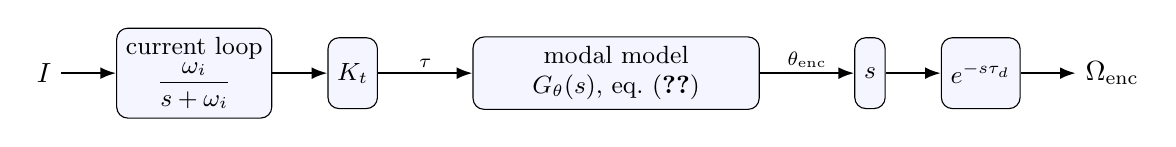
\begin{tikzpicture}[node distance=7mm]
\node (i) {$I$};
\node[blk, right=of i] (cl) {current loop\\ $\dfrac{\omega_i}{s+\omega_i}$};
\node[blk, right=of cl] (kt) {$K_t$};
\node[blk, right=12mm of kt, text width=3.4cm] (mech) {modal model\\ $G_\theta(s)$, eq.~\eqref{eq:modalfrf}};
\node[blk, right=12mm of mech] (der) {$s$};
\node[blk, right=of der] (del) {$e^{-s\tau_d}$};
\node[right=of del] (o) {$\Omega_\mathrm{enc}$};
\draw[sig] (i) -- (cl); \draw[sig] (cl) -- (kt); \draw[sig] (kt) -- node[above, lab]{$\tau$} (mech);
\draw[sig] (mech) -- node[above, lab]{$\theta_\mathrm{enc}$} (der); \draw[sig] (der) -- (del); \draw[sig] (del) -- (o);
\end{tikzpicture}
\caption{Plant measured by WorkBench as modelled in~\eqref{eq:plant}.}\label{fig:plant}
\end{figure}

\subsection{Elevation: H7 with two modal masses on the motor stator, rigid telescope}\label{sec:elev}
\paragraph{Rotor chain.} H7 elevation block with the telescope rigidly attached to the ring, i.e.\ fused with the hub centre (Figure~\ref{fig:elev}). Four rotor nodes remain: encoder disc $e$, hub with telescope $hp$, motor rotor $m$, rear end of the shaft (rear). Their inertias and the three shaft stiffnesses $k_{\theta1}$ ($e$--$hp$), $k_{\theta2}$ ($hp$--$m$) and $k_{\theta3}$ ($m$--rear) are the CAD/H7 values multiplied by factors $s_{(\cdot)}\in[0.80,1.20]$.

\paragraph{Stator masses.} Each fork mode excited by the stator is a modal oscillator $q_r$ ($r=1,2$):
\begin{itemize}
\item modal inertia $J_r$ and stiffness $k_r^s=J_r(2\pi f_r)^2$ to the ground;
\item excited by the stator reaction $-\tau$ with unit participation;
\item it moves the encoder head by $\kappa_rq_r$, so that the encoder reads $\theta_\mathrm{enc}=\theta_e-\sum_r\kappa_rq_r$.
\end{itemize}
Only the residue $a_r=\kappa_r/J_r$ is identifiable. With the convention $|\kappa_r|=1$, $J_r=1/|a_r|$ and $\kappa_r=\mathrm{sign}(a_r)$. A negative $a_r$ means that in that mode the encoder head moves against the stator.

\paragraph{Bearings.} The polar bearings join the hub to the stator structure, whose rotation is the modal superposition $\varphi_s=q_1+q_2$: $\mathbf v=\mathbf e_{hp}-\mathbf e_{q_1}-\mathbf e_{q_2}$.

\paragraph{Input and output.}
\begin{equation}
\mathbf x=[\theta_e,\theta_{hp},\theta_m,\theta_\mathrm{rear},q_1,q_2]^T,\qquad \mathbf e=\mathbf e_m-\mathbf e_{q_1}-\mathbf e_{q_2},\qquad \mathbf c=\mathbf e_e-\kappa_1\mathbf e_{q_1}-\kappa_2\mathbf e_{q_2} .
\end{equation}

\begin{figure}[H]\centering
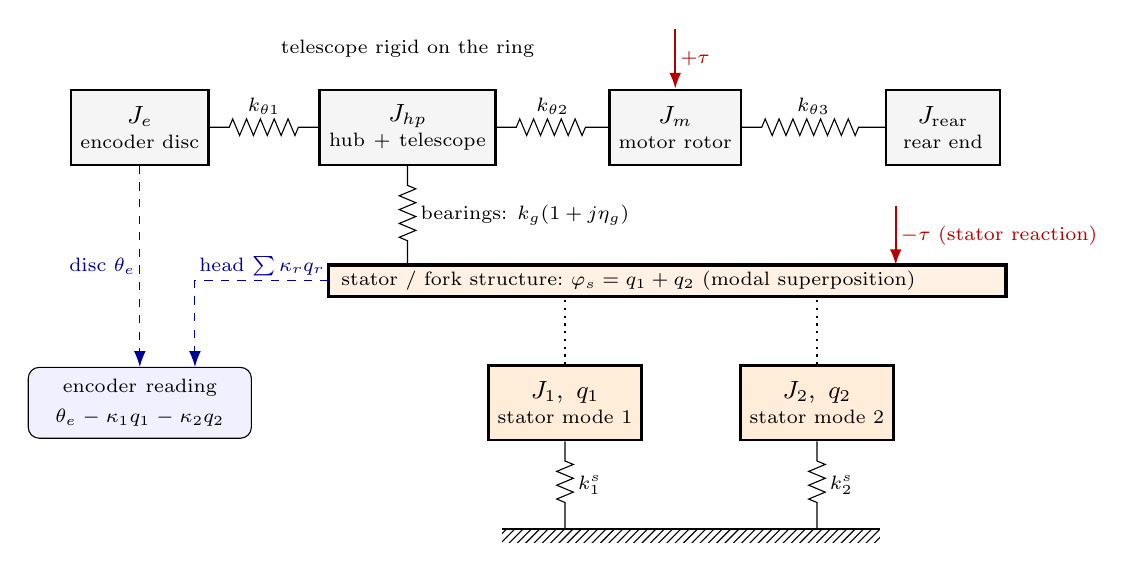
\begin{tikzpicture}[x=1cm, y=1cm]
\node[mass] (e) at (0,0) {$J_e$\\[-2pt]\scriptsize encoder disc};
\node[mass, text width=2.0cm] (h) at (3.4,0) {$J_{hp}$\\[-2pt]\scriptsize hub + telescope};
\node[mass] (m) at (6.8,0) {$J_m$\\[-2pt]\scriptsize motor rotor};
\node[mass] (r) at (10.2,0) {$J_\mathrm{rear}$\\[-2pt]\scriptsize rear end};
\draw[spring] (e.east) -- node[above=3pt, lab]{$k_{\theta1}$} (h.west);
\draw[spring] (h.east) -- node[above=3pt, lab]{$k_{\theta2}$} (m.west);
\draw[spring] (m.east) -- node[above=3pt, lab]{$k_{\theta3}$} (r.west);
\draw[sig, red!70!black] (6.8,1.25) -- node[right, lab, red!70!black]{$+\tau$} (m.north);
\node[lab, align=center] at (3.4,1.0) {telescope rigid on the ring};
\draw[very thick, fill=orange!10] (2.4,-2.15) rectangle (11.0,-1.75);
\node[lab, anchor=west] at (2.5,-1.95) {stator / fork structure:\ $\varphi_s=q_1+q_2$ (modal superposition)};
\draw[spring] (h.south) -- node[right=3pt, lab]{bearings: $k_g(1+j\eta_g)$} (3.4,-1.75);
\draw[sig, red!70!black] (9.6,-1.0) -- node[right, lab, red!70!black]{$-\tau$ (stator reaction)} (9.6,-1.75);
\node[mass, fill=orange!15] (q1) at (5.4,-3.5) {$J_1,\ q_1$\\[-2pt]\scriptsize stator mode 1};
\node[mass, fill=orange!15] (q2) at (8.6,-3.5) {$J_2,\ q_2$\\[-2pt]\scriptsize stator mode 2};
\draw[dotted, thick] (q1.north) -- (5.4,-2.15); \draw[dotted, thick] (q2.north) -- (8.6,-2.15);
\draw[spring] (q1.south) -- node[right=3pt, lab]{$k_1^s$} (5.4,-5.1);
\draw[spring] (q2.south) -- node[right=3pt, lab]{$k_2^s$} (8.6,-5.1);
\ground{4.6}{9.4}{-5.1}
\node[blk, fill=blue!6, text width=2.6cm] (enc) at (0,-3.5) {\scriptsize encoder reading\\ $\theta_e-\kappa_1q_1-\kappa_2q_2$};
\draw[meas] (e.south) -- node[left, lab]{disc $\theta_e$} (enc.north);
\draw[meas] (2.4,-1.95) -| node[pos=0.25, above, lab]{head $\sum\kappa_r q_r$} ($(enc.north)+(0.7,0)$);
\end{tikzpicture}
\caption{Elevation model (translational analogue). Grey: rotor chain of H7 with the telescope fused with the hub; orange: stator structure and its two modal oscillators. The damping is not drawn: it is introduced mode by mode (Section~\ref{sec:modal}), apart from the hysteretic part of the bearings.}\label{fig:elev}
\end{figure}

\subsection{Azimuth: flexible load, rigid telescope}\label{sec:azmodel}
The H7 azimuth load (fork, hub and ring, $J_\mathrm{load}$ from CAD) is split into a fork base $L$ and a fork top, joined by a stiffness $k_{LA}$ introduced in the model (Figure~\ref{fig:az}). The telescope is rigid on the ring, so it is fused with the fork top, which carries the hub and the ring:
\begin{equation}
J_L=(1-\alpha)\,s_{J_L}J_\mathrm{load},\qquad J_{AP}=\alpha\,s_{J_L}J_\mathrm{load}+s_{J_L}J_P .
\end{equation}
\begin{itemize}
\item One CAD factor $s_{J_L}$ scales the load and the telescope together. Only $J_L$ and $J_{AP}$ affect the response, so two separate factors would not be identifiable together with $\alpha$.
\item The encoder and motor rotors and the shafts $k_1$ ($e$--$m$) and $k_2$ ($m$--$L$) are the CAD/H7 values times factors in $[0.80,1.20]$.
\item The bearings ground the fork base: $\mathbf v=\mathbf e_L$.
\item $\mathbf x=[\psi_e,\psi_m,\psi_L,\psi_{AP}]^T$, $\mathbf e=\mathbf e_m$, $\mathbf c=\mathbf e_e$.
\end{itemize}

\begin{figure}[H]\centering
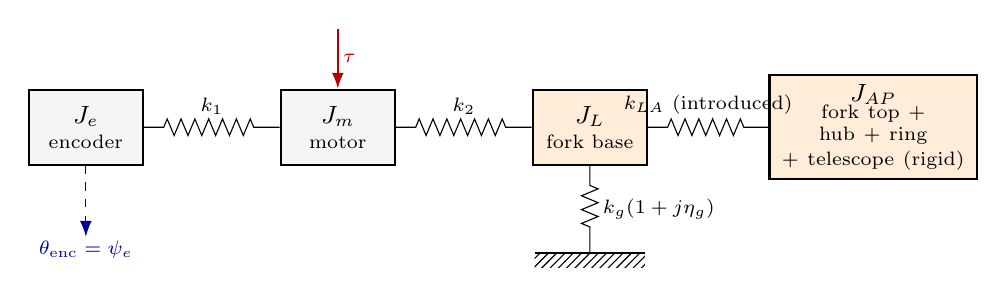
\begin{tikzpicture}[x=1cm, y=1cm]
\node[mass] (e) at (0,0) {$J_e$\\[-2pt]\scriptsize encoder};
\node[mass] (m) at (3.2,0) {$J_m$\\[-2pt]\scriptsize motor};
\node[mass, fill=orange!15] (L) at (6.4,0) {$J_L$\\[-2pt]\scriptsize fork base};
\node[mass, fill=orange!15, text width=2.4cm] (A) at (10.0,0) {$J_{AP}$\\[-2pt]\scriptsize fork top + hub + ring\\[-2pt]\scriptsize + telescope (rigid)};
\draw[spring] (e.east) -- node[above=3pt, lab]{$k_1$} (m.west);
\draw[spring] (m.east) -- node[above=3pt, lab]{$k_2$} (L.west);
\draw[spring] (L.east) -- node[above=3pt, lab]{$k_{LA}$ (introduced)} (A.west);
\draw[spring] (L.south) -- node[right=3pt, lab]{$k_g(1+j\eta_g)$} (6.4,-1.6);
\ground{5.7}{7.1}{-1.6}
\draw[sig, red!70!black] (3.2,1.25) -- node[right, lab, red!70!black]{$\tau$} (m.north);
\draw[meas] (e.south) -- ++(0,-0.9) node[below, lab]{$\theta_\mathrm{enc}=\psi_e$};
\end{tikzpicture}
\caption{Azimuth model (translational analogue). Orange: the H7 load node split into fork base and fork top; the telescope is rigid on the ring and moves with the fork top.}\label{fig:az}
\end{figure}

%% ===================================================================================================
\section{Modal formulation}\label{sec:modal}
\paragraph{Modes.} The undamped eigenproblem of each axis uses the real stiffness, including the real part of the bearings:
\begin{equation}
\mathbf K\bm\phi_k=\omega_k^2\,\mathbf M\bm\phi_k,\qquad \bm\Phi=[\bm\phi_1,\dots,\bm\phi_n],\qquad \bm\Phi^T\mathbf M\bm\Phi=\mathbf I,\qquad \bm\Phi^T\mathbf K\bm\Phi=\bm\Omega^2=\mathrm{diag}(\omega_k^2) .
\end{equation}
All the $n$ modes are kept (6 in elevation, 4 in azimuth), so the modal formulation is exact and there is no truncation.

\paragraph{Damping.} With $\mathbf x=\bm\Phi\mathbf z$, each mode $k$ receives its own viscous modal damping $\zeta_k$, a fitted parameter bounded by $\zeta_k\leq\zetaMax$. The hysteretic part of the bearings is projected on the modal coordinates without approximation:
\begin{equation}
\Bigl(s^2\mathbf I+s\,\mathrm{diag}(2\zeta_k\omega_k)+\bm\Omega^2+j\,h\,\mathbf w\mathbf w^T\Bigr)\mathbf z=\mathbf b\,\tau,\qquad
\mathbf w=\bm\Phi^T\mathbf v,\quad \mathbf b=\bm\Phi^T\mathbf e,\quad \mathbf g=\bm\Phi^T\mathbf c .\label{eq:modaleq}
\end{equation}
The modal viscous damping is diagonal: every mode is an independent second-order system. The bearings add a rank-one coupling, because they act on one deflection $\mathbf v^T\mathbf x=\mathbf w^T\mathbf z$. Their loss factor $\eta_g$ is not a modal damping ratio, so it is not subject to the limit on $\zeta_k$ (as prescribed, the bearings remain a linear hysteretic element).

\paragraph{Frequency response.} With $D_k(s)=s^2+2\zeta_k\omega_ks+\omega_k^2$ and the Sherman--Morrison formula for the rank-one term:
\begin{equation}
G_\theta(s)=\underbrace{\sum_{k=1}^{n}\frac{R_k}{D_k(s)}}_{\text{modal superposition}}
-\;\frac{j\,h\,\Bigl(\sum_k\dfrac{g_kw_k}{D_k}\Bigr)\Bigl(\sum_k\dfrac{w_kb_k}{D_k}\Bigr)}{1+j\,h\displaystyle\sum_k\frac{w_k^2}{D_k}},\qquad R_k=g_kb_k=(\mathbf c^T\bm\phi_k)(\bm\phi_k^T\mathbf e) .\label{eq:modalfrf}
\end{equation}
\begin{itemize}
\item $R_k$ is the \emph{modal residue}: how strongly mode $k$ is driven by the motor torque and seen by the encoder. Positive for a collocated mode, negative where the encoder head moves against the stator.
\item To first order the bearings give mode $k$ the hysteretic modal loss factor $\eta_k=h\,w_k^2/\omega_k^2$, reported in the mode tables. It is large only for the mode in which the axis turns on the bearings.
\item This formulation was checked against the direct solution of~\eqref{eq:lumped}: they agree to $10^{-7}$ in relative terms.
\end{itemize}

\paragraph{Sign of the residues and non-minimum-phase zeros.} On the elevation axis, with a rigid rotor of inertia $J$ and the two stator modes undamped,
\begin{equation}
G_\theta\simeq\frac{1}{Js^2}+\frac{a_1}{s^2+\omega_1^2}+\frac{a_2}{s^2+\omega_2^2}=\frac{Au^2+Bu+C}{s^2(s^2+\omega_1^2)(s^2+\omega_2^2)},\quad u=s^2,
\end{equation}
\begin{equation}
A=\frac1J+a_1+a_2,\quad B=\frac{\omega_1^2+\omega_2^2}J+a_1\omega_2^2+a_2\omega_1^2,\quad C=\frac{\omega_1^2\omega_2^2}J .
\end{equation}
\begin{itemize}
\item \textbf{Collocated residues} ($a_r>0$): the zeros interlace with the poles on the imaginary axis.
\item \textbf{Negative residue and $B^2-4AC<0$}: the zeros form a quartet $\pm\sigma\pm j\omega$, one pair in the right half-plane. Relative to a collocated pattern this adds a phase drop of 360$^\circ$.
\item \textbf{The farther $B^2-4AC$ is below zero}, the farther the quartet is from the imaginary axis. Close to zero, the quartet behaves as a lightly damped antiresonance.
\end{itemize}

%% ===================================================================================================
\section{Identification}\label{sec:method}
\begin{figure}[H]\centering
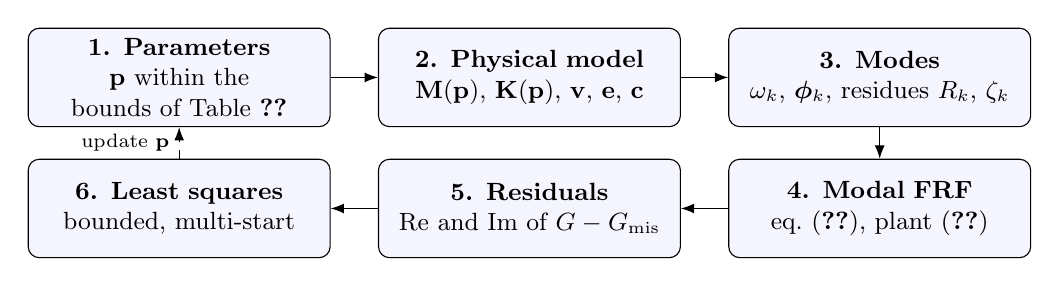
\begin{tikzpicture}[node distance=4mm and 6mm, every node/.style={font=\small},
  box/.style={draw, rounded corners, align=center, text width=3.6cm, minimum height=1.25cm, fill=blue!4}]
\node[box] (a) {\textbf{1. Parameters}\\ $\mathbf p$ within the bounds of Table~\ref{tab:constraints}};
\node[box, right=of a] (b) {\textbf{2. Physical model}\\ $\mathbf M(\mathbf p)$, $\mathbf K(\mathbf p)$, $\mathbf v$, $\mathbf e$, $\mathbf c$};
\node[box, right=of b] (c) {\textbf{3. Modes}\\ $\omega_k$, $\bm\phi_k$, residues $R_k$, $\zeta_k$};
\node[box, below=of c] (d) {\textbf{4. Modal FRF}\\ eq.~\eqref{eq:modalfrf}, plant~\eqref{eq:plant}};
\node[box, left=of d] (e) {\textbf{5. Residuals}\\ $\mathrm{Re}$ and $\mathrm{Im}$ of $G-G_\mathrm{mis}$};
\node[box, left=of e] (f) {\textbf{6. Least squares}\\ bounded, multi-start};
\draw[-{Latex}] (a) -- (b); \draw[-{Latex}] (b) -- (c); \draw[-{Latex}] (c) -- (d); \draw[-{Latex}] (d) -- (e); \draw[-{Latex}] (e) -- (f);
\draw[-{Latex}, dashed] (f.north) -- node[left, font=\scriptsize]{update $\mathbf p$} (a.south);
\end{tikzpicture}
\caption{Identification loop, run separately for the two axes by \texttt{analisi\_forcella\_modale.py} (model in \texttt{src/gimbal\_mdof/forcella\_modale.py}).}\label{fig:flow}
\end{figure}

\subsection{Residuals and cost}
At every measured frequency $f_i$ of every measurement of the axis, the residual is the difference of the real parts and the difference of the imaginary parts of the plant:
\begin{equation}
r_i^{\mathrm{Re}}(\mathbf p)=w_i\,\mathrm{Re}\bigl[G(j\omega_i;\mathbf p)-G_\mathrm{mis}(j\omega_i)\bigr],\qquad
r_i^{\mathrm{Im}}(\mathbf p)=w_i\,\mathrm{Im}\bigl[G(j\omega_i;\mathbf p)-G_\mathrm{mis}(j\omega_i)\bigr],
\end{equation}
and the parameters minimise the sum of their squares:
\begin{equation}
\hat{\mathbf p}=\arg\min_{\mathbf p_\mathrm{lo}\leq\mathbf p\leq\mathbf p_\mathrm{hi}}F(\mathbf p),\qquad
F(\mathbf p)=\frac12\sum_i\Bigl[\bigl(r_i^{\mathrm{Re}}\bigr)^2+\bigl(r_i^{\mathrm{Im}}\bigr)^2\Bigr]=\frac12\sum_iw_i^2\,\bigl|G(j\omega_i;\mathbf p)-G_\mathrm{mis}(j\omega_i)\bigr|^2 .
\end{equation}
\begin{itemize}
\item The error is the complex distance between model and measurement in the Nyquist plane, in (rad/s)/A, with a quadratic loss: no logarithm and no robust loss.
\item Every point counts with its absolute size. The cost is therefore dominated by the points of large magnitude: the low-frequency region (1--10\,Hz, about $-40$\,dB) and the resonance peaks. Points near $-65$\,dB at 150\,Hz weigh about $10^3$ times less.
\item The only weight is $w_i=\sqrt{\Delta\ln f_i/0.01}$, the width in $\ln f$ that each point represents. It makes the sum an integral over $\ln f$, so that the finer grids (1\,\%) and the overlapping elevation measurements do not count more than a coarser grid over the same band.
\end{itemize}

\subsection{Parameters and constraints}
\begin{table}[H]\centering\small
\caption{Parameter classes and constraints. The CAD factors multiply the CAD/H7 value of the corresponding inertia or stiffness.}\label{tab:constraints}
\begin{tabular}{L{3.4cm}L{6.0cm}L{6.2cm}}\toprule
class & elevation & azimuth \\ \midrule
CAD inertias, $[0.80,1.20]$ & $s_{J_e}$, $s_{J_{hp}}$ (hub + telescope), $s_{J_m}$, $s_{J_\mathrm{rear}}$ & $s_{J_e}$, $s_{J_m}$, $s_{J_L}$ (load + telescope) \\
CAD stiffnesses, $[0.80,1.20]$ & $s_{k_{\theta1}}$, $s_{k_{\theta2}}$, $s_{k_{\theta3}}$ (shafts) & $s_{k_1}$, $s_{k_2}$ (shafts) \\
ground (bearings), free & $k_g\in[1,10^6]$\,N\,m/rad, $\eta_g\in[10^{-3},30]$ & $k_g\in[1,10^6]$\,N\,m/rad, $\eta_g\in[10^{-3},30]$ \\
introduced in the model, free & -- (telescope rigid on the ring) & $k_{LA}\in[10^3,10^8]$\,N\,m/rad, $\alpha\in[0.02,0.98]$ \\
stator masses, free & $f_1\in[40,80]$, $f_2\in[80,140]$\,Hz; $a_r\in[-50,50]$\,(kg\,m$^2$)$^{-1}$ & -- \\
modal damping & $\zeta_1\dots\zeta_6\in[10^{-4},\zetaMax]$ & $\zeta_1\dots\zeta_4\in[10^{-4},\zetaMax]$ \\
drive and motor & $\tau_d\in[10^{-6},2\times10^{-3}]$\,s; $g_{K_t}\in[\ktLo,\ktHi]$ & $\tau_d\in[10^{-6},2\times10^{-3}]$\,s; $g_{K_t}\in[\ktLo,\ktHi]$ \\ \bottomrule
\end{tabular}\end{table}
\begin{itemize}
\item The positive parameters are searched on their logarithm, the CAD factors, $\alpha$ and the residues on their value.
\item The damping ratios of the stator masses are the $\zeta_k$ of the corresponding global modes. The coupling through the bearings is weak, so those modes are the stator oscillators to within $10^{-3}$ in their shapes.
\item The ranges of $f_1$ and $f_2$ keep the two stator masses in their order. They are wide compared with the measured resonances (56--59 and 99--100\,Hz).
\end{itemize}

\subsection{Solver, starts and uncertainty}
\begin{itemize}
\item \textbf{Solver.} Bounded trust-region least squares (\texttt{scipy.optimize.least\_squares}, quadratic loss, Jacobian scaling), at most 3000 evaluations per start. The start with the lowest cost is kept.
\item \textbf{Starts, elevation} (\nStartsP). First, the fourth-step result (CAD $\pm\cadJ$\,\%) with $g_{K_t}=1$. As a check, also the first-step result and every combination of the signs of $a_1,a_2$ with $|a_r|\in\{0.3,1.5\}$, with CAD factors at 1, $\zeta_k=0.005$, and $k_g$, $\eta_g$, $\tau_d$, $f_r$ from the first step.
\item \textbf{Starts, azimuth} (\nStartsA). First, the fourth-step result with $g_{K_t}=1$; as a check, the first-step result and $\alpha\in\{0.2,0.4,0.7\}$ with $k_{LA}$ placing the base--top mode at 49 or 56\,Hz.
\item The column ``start'' of the parameter tables lists the values used over all the starts.
\item \textbf{Uncertainty.} $\mathrm{cov}=s^2(\mathbf J_f^T\mathbf J_f)^{+}$, with $s^2=2F/(m-n_f)$, where $\mathbf J_f$ is the Jacobian restricted to the $n_f$ parameters not at a bound. A parameter at a bound is fixed by the constraint and has no standard deviation; ``n.d.'' marks a free parameter that the data do not see.
\end{itemize}

\paragraph{Goodness measures.} As in the first step, on the measured points of the band:
\begin{itemize}
\item the NRMSE fit on the complex response, $\mathrm{fit}=100\bigl(1-\lVert G_\mathrm{mis}-G\rVert/\lVert G_\mathrm{mis}-\overline{G_\mathrm{mis}}\rVert\bigr)\,\%$, over 1--150\,Hz and in 1--5, 5--100 and 100--150\,Hz;
\item the rms of $20\log_{10}|G/G_\mathrm{mis}|$ (dB) and of the phase error (deg).
\end{itemize}
The NRMSE measures the same complex distance that the fit minimises. The rms in dB and degrees weighs all the points alike, so it shows the errors at small magnitude that the cost does not see.

%% ===================================================================================================
\section{Results: elevation}\label{sec:res_elev}
All \nStartsP\ starts end at the same cost (\costP, against \costPStepJ\ in the third step and \costPStep\ in the second): the minimum does not depend on the start. \nBoundP\ of the \nParP\ parameters end at a bound (\boundP).

\begin{table}[H]\centering\scriptsize\setlength{\tabcolsep}{3pt}
\caption{Elevation: fitted parameters. CAD: value of the quantity that a factor scales; physical: factor times CAD. Std: relative standard deviation of the free parameters.}\label{tab:polar_params}
\begin{tabular}{lL{1.8cm}lrrL{2.2cm}L{1.7cm}lrl}\toprule
param. & class & unit & estimate & CAD & physical & start & bounds & std & at bound \\ \midrule
$s_{J_e}$ & CAD, $\pm20$\,\% & -- & 1.2 & \ensuremath{8.94\times10^{-6}} & \ensuremath{1.07\times10^{-5}} kg\,m$^2$ & 1, 1.2 & [0.8, 1.2] & -- & yes \\
$s_{J_{hp}}$ & CAD, $\pm20$\,\% & -- & 1.177 & 0.898 & 1.06 kg\,m$^2$ & 1, 1.17 & [0.8, 1.2] & n.d. &  \\
$s_{J_m}$ & CAD, $\pm20$\,\% & -- & 1.2 & 0.000657 & 0.000788 kg\,m$^2$ & 1, 1.2 & [0.8, 1.2] & -- & yes \\
$s_{J_\mathrm{rear}}$ & CAD, $\pm20$\,\% & -- & 1.2 & 0.000644 & 0.000773 kg\,m$^2$ & 1, 1.2 & [0.8, 1.2] & -- & yes \\
$s_{k_{\theta1}}$ & CAD, $\pm20$\,\% & -- & 0.8 & \ensuremath{4.67\times10^{4}} & \ensuremath{3.74\times10^{4}} N\,m/rad & 0.8, 1 & [0.8, 1.2] & -- & yes \\
$s_{k_{\theta2}}$ & CAD, $\pm20$\,\% & -- & 0.8 & \ensuremath{1.01\times10^{4}} & \ensuremath{8.09\times10^{3}} N\,m/rad & 0.8, 1 & [0.8, 1.2] & -- & yes \\
$s_{k_{\theta3}}$ & CAD, $\pm20$\,\% & -- & 0.8 & \ensuremath{9.69\times10^{3}} & \ensuremath{7.76\times10^{3}} N\,m/rad & 0.8, 1 & [0.8, 1.2] & -- & yes \\
$k_g$ & ground, free & N\,m/rad & 129.4 & -- & -- & 117, 129 & [1, \ensuremath{1\times10^{6}}] & n.d. &  \\
$\eta_g$ & ground, free & -- & 2.722 & -- & -- & 2.72, 3.2 & [0.001, 30] & 660.8\,\% &  \\
$\tau_d$ & drive & s & 0.000211 & -- & -- & 0.000211, 0.000595 & [\ensuremath{1\times10^{-6}}, 0.002] & 39.9\,\% &  \\
$f_1$ & stator mass, free & Hz & 56.69 & -- & -- & 56.7, 57.7 & [40, 80] & 0.3\,\% &  \\
$a_1$ & stator mass, free & 1/(kg\,m$^2$) & $-$0.5664 & -- & -- & $\pm0.3$, $\pm0.5701$, $\pm0.6948$, $\pm1.5$ & [$-$50, 50] & n.d. &  \\
$f_2$ & stator mass, free & Hz & 99.02 & -- & -- & 99, 100 & [80, 140] & 0.3\,\% &  \\
$a_2$ & stator mass, free & 1/(kg\,m$^2$) & 0.6496 & -- & -- & $\pm0.3$, $\pm0.6264$, $\pm0.6539$, $\pm1.5$ & [$-$50, 50] & n.d. &  \\
$g_{K_t}$ & motor, $\pm10$\,\% & -- & 1.007 & -- & -- & 1 & [0.9, 1.1] & n.d. &  \\
$\zeta_1$ & modal, $\leq0.05$ & -- & 0.0001 & -- & -- & 0.0001, 0.005 & [0.0001, 0.05] & -- & yes \\
$\zeta_2$ & modal, $\leq0.05$ & -- & 0.03299 & -- & -- & 0.005, 0.033 & [0.0001, 0.05] & 6.9\,\% &  \\
$\zeta_3$ & modal, $\leq0.05$ & -- & 0.0327 & -- & -- & 0.005, 0.0327 & [0.0001, 0.05] & 10.3\,\% &  \\
$\zeta_4$ & modal, $\leq0.05$ & -- & 0.05 & -- & -- & 0.005, 0.05 & [0.0001, 0.05] & -- & yes \\
$\zeta_5$ & modal, $\leq0.05$ & -- & 0.05 & -- & -- & 0.005, 0.05 & [0.0001, 0.05] & -- & yes \\
$\zeta_6$ & modal, $\leq0.05$ & -- & 0.05 & -- & -- & 0.005, 0.05 & [0.0001, 0.05] & -- & yes
\\ \bottomrule
\end{tabular}\end{table}

\begin{table}[H]\centering\small\setlength{\tabcolsep}{4pt}
\caption{Elevation: modes of the fitted model. $R_k$: modal residue [1/(kg\,m$^2$)]; $\eta_k$: hysteretic loss factor given by the bearings; shapes normalised on the largest node.}\label{tab:polar_modes}
\begin{tabular}{lrrrrrrrrrr}\toprule
mode & $f_k$ [Hz] & $\zeta_k$ & $R_k$ & $\eta_k$ & $e$ & $hp$ & $m$ & rear & $q_1$ & $q_2$ \\ \midrule
1 & 1.8 & 0.0001 & 0.944 & 2.7 & +1.00 & +1.00 & +1.00 & +1.00 & +0.00 & +0.00 \\
2 & 56.7 & 0.0330 & $-$0.566 & 0.0016 & $-$0.00 & $-$0.00 & $-$0.00 & $-$0.00 & +1.00 & $-$0.00 \\
3 & 99.0 & 0.0327 & 0.65 & 0.00059 & $-$0.00 & $-$0.00 & $-$0.00 & $-$0.00 & +0.00 & +1.00 \\
4 & 315.8 & 0.0500 & $-$0.676 & \ensuremath{1.2\times10^{-7}} & $-$0.00 & $-$0.00 & +0.61 & +1.00 & +0.00 & +0.00 \\
5 & 814.9 & 0.0500 & $-$0.271 & \ensuremath{1.1\times10^{-9}} & $-$0.00 & $-$0.00 & +1.00 & $-$0.62 & +0.00 & +0.00 \\
6 & 9395.0 & 0.0500 & 0.0028 & \ensuremath{9.7\times10^{-13}} & +1.00 & $-$0.00 & +0.00 & $-$0.00 & +0.00 & +0.00
\\ \bottomrule
\end{tabular}\end{table}

\paragraph{Modes.}
\begin{itemize}
\item \textbf{Mode 1, \fBearP\,Hz}: the whole axis turns on the bearings. Its damping is the hysteretic one of the bearings ($\eta_1=\etaBearP$); its viscous $\zeta_1$ goes to the lower bound.
\item \textbf{Modes 2 and 3}: the stator masses, at \fMassI\ and \fMassII\,Hz, with $\zeta=\zMassI$ and \zMassII, inside the bounds. The residues are $a_1=\aMassI$ and $a_2=\aMassII$\,(kg\,m$^2$)$^{-1}$: \aStepI\ and \aStepII\ in the second step ($\zeta$ at the bound \zetaMaxStep), \aLogI\ and \aLogII\ in the first step ($\zeta=\zLogI$ and \zLogII).
\item \textbf{Modes 4--6}: shaft and encoder modes at \fShaftP\,Hz, \fShaftPb\,Hz and about 10\,kHz, outside the band. They act as residual stiffness and mass terms. The damping of modes 4 and 5 goes to the upper bound, but it has no visible effect in the band: there these modes contribute almost only their static term $R_k/\omega_k^2$.
\end{itemize}

\paragraph{Bearings.} $k_g=\kg$\,N\,m/rad and $\eta_g=\etag$, against \kgStep\ and \etagStep\ in the second step and \kgPrev\ and \etagPrev\ in the first. The low-frequency part is robust to the change of method and of the damping limit.

\paragraph{Parameters at a bound.}
\begin{itemize}
\item The CAD factors of encoder, motor and rear end reach $+\cadJ$\,\%, the shafts $-\cadK$\,\%. The hub--telescope factor stops inside the bounds, $s_{J_{hp}}=\sJhpP$.
  \begin{itemize}
  \item The diagnostic with $\pm50$\,\% (Section~\ref{sec:quality}) gives the same cost (within \cadCostP\,\%) with different factors.
  \item The cost is flat along these directions: the data do not determine the CAD factors of the elevation chain, and the bounds settle them.
  \end{itemize}
\item In the second step the delay went to its lower bound; here it is free but poorly determined (Table~\ref{tab:polar_params}).
\item $g_{K_t}=\gKtP$ and $s_{J_{hp}}=\sJhpP$ are both inside their bounds, but only their ratio is determined by the data: their standard deviations are not defined (``n.d.''). The elevation is consistent with the catalogue $K_t$.
\end{itemize}

\begin{figure}[H]\centering
\includegraphics[width=\linewidth]{figures/polar_bode.pdf}
\caption{Elevation plant [dB (rad/s)/A] and phase [deg] in the fit band: the three measurements and the modal model. Right: zoom 40--150\,Hz.}\label{fig:polar_bode}
\end{figure}

\paragraph{Effect of the damping limit} (Figure~\ref{fig:polar_bode}).
\begin{itemize}
\item \textbf{Peaks.} The height of a modal peak grows as $|R_k|/\zeta_k$. In the second step $\zeta$ was held at \zetaMaxStep, about a third of the value the data ask for, and the least squares lowered the residues to \aStepI\ and \aStepII\ to contain the peaks. Here $\zeta$ and the residues are both free to take the values the data ask for, and the peaks of the two nominal measurements are matched in height and width. The 16-screw measurement has a higher first peak, about 3\,dB above the model.
\item \textbf{Antiresonance near 70\,Hz.} With the residues of the second step, $B^2-4AC=$\,\nmpDiscStep\ was only slightly negative and the quartet of zeros lay near the imaginary axis ($\approx\nmpFStep$\,Hz, $\zeta\approx\pm\nmpZetaStep$ in the undamped approximation), which produced a deep antiresonance near 70\,Hz that the measurement does not have. With the present residues $B^2-4AC=$\,\nmpDisc\ and the quartet moves away from the axis ($\approx\nmpF$\,Hz, $\zeta\approx\pm\nmpZeta$): the response between the two modes is smooth, as measured.
\item \textbf{Why raising the damping alone would not help.} With the second-step residues kept fixed, raising $\zeta_2,\zeta_3$ up to about 0.05 makes that antiresonance deeper, not shallower. The modal damping splits the quartet asymmetrically: it moves the left-half-plane pair away from the axis and the right-half-plane pair towards it. The antiresonance disappears because the larger damping allows larger residues, not because of the damping itself.
\item \textbf{Phase.} Above 100\,Hz the model phase matches the measurement. Between 60 and 95\,Hz it lies about 10--20$^\circ$ above the measurement.
\item \textbf{Below 30\,Hz} the model stays a few dB below the measurement between 9 and 30\,Hz. This region contains the unmodelled pair at 8--9\,Hz (Section~\ref{sec:limits}) and is unchanged from the second step.
\end{itemize}

\begin{figure}[H]\centering
\includegraphics[width=0.92\linewidth]{figures/polar_modal_terms.pdf}
\caption{Elevation: modal terms $R_k/D_k(s)$ of~\eqref{eq:modalfrf} and the rank-one bearing term, each with the plant factors of~\eqref{eq:plant}. Grey dots: 1--600\,Hz measurement in the band.}\label{fig:polar_terms}
\end{figure}

%% ===================================================================================================
\section{Results: azimuth}\label{sec:res_az}
All \nStartsA\ starts reach the same cost (\costA, against \costAStepJ\ in the third step and \costAStep\ in the second). \nBoundA\ of the \nParA\ parameters end at a bound (\boundA).

\begin{table}[H]\centering\scriptsize\setlength{\tabcolsep}{3pt}
\caption{Azimuth: fitted parameters. CAD: value of the quantity that a factor scales ($s_{J_L}$: load plus telescope); physical: factor times CAD. Std: relative standard deviation of the free parameters.}\label{tab:az_params}
\begin{tabular}{lL{1.8cm}lrrL{2.2cm}L{1.7cm}lrl}\toprule
param. & class & unit & estimate & CAD & physical & start & bounds & std & at bound \\ \midrule
$s_{J_e}$ & CAD, $\pm20$\,\% & -- & 0.8 & 0.000185 & 0.000148 kg\,m$^2$ & 0.8, 1 & [0.8, 1.2] & -- & yes \\
$s_{J_m}$ & CAD, $\pm20$\,\% & -- & 0.8 & 0.000212 & 0.00017 kg\,m$^2$ & 0.8, 1 & [0.8, 1.2] & -- & yes \\
$s_{J_L}$ & CAD, $\pm20$\,\% & -- & 1.2 & 2.16 & 2.6 kg\,m$^2$ & 1, 1.2 & [0.8, 1.2] & -- & yes \\
$s_{k_1}$ & CAD, $\pm20$\,\% & -- & 1.2 & \ensuremath{9.55\times10^{3}} & \ensuremath{1.15\times10^{4}} N\,m/rad & 1, 1.2 & [0.8, 1.2] & -- & yes \\
$s_{k_2}$ & CAD, $\pm20$\,\% & -- & 1.2 & \ensuremath{1.31\times10^{4}} & \ensuremath{1.57\times10^{4}} N\,m/rad & 1, 1.2 & [0.8, 1.2] & -- & yes \\
$\alpha$ & introduced, free & -- & 0.6249 & -- & -- & 5 values & [0.02, 0.98] & 1.9\,\% &  \\
$k_{LA}$ & introduced, free & N\,m/rad & \ensuremath{5.607\times10^{4}} & -- & -- & 8 values & [\ensuremath{1\times10^{3}}, \ensuremath{1\times10^{8}}] & 2.3\,\% &  \\
$k_g$ & ground, free & N\,m/rad & 1015 & -- & -- & 914, \ensuremath{1.01\times10^{3}} & [1, \ensuremath{1\times10^{6}}] & 1.2\,\% &  \\
$\eta_g$ & ground, free & -- & 0.5126 & -- & -- & 0.576, 0.645 & [0.001, 30] & 2.6\,\% &  \\
$\tau_d$ & drive & s & 0.0004786 & -- & -- & 0.000453, 0.00048 & [\ensuremath{1\times10^{-6}}, 0.002] & 4.3\,\% &  \\
$g_{K_t}$ & motor, $\pm10$\,\% & -- & 0.9 & -- & -- & 1 & [0.9, 1.1] & -- & yes \\
$\zeta_1$ & modal, $\leq0.05$ & -- & 0.0001 & -- & -- & 0.0001, 0.005 & [0.0001, 0.05] & -- & yes \\
$\zeta_2$ & modal, $\leq0.05$ & -- & 0.02801 & -- & -- & 0.005, 0.0302 & [0.0001, 0.05] & 6.2\,\% &  \\
$\zeta_3$ & modal, $\leq0.05$ & -- & 0.0001 & -- & -- & 0.0001, 0.005 & [0.0001, 0.05] & -- & yes \\
$\zeta_4$ & modal, $\leq0.05$ & -- & 0.05 & -- & -- & 0.005, 0.05 & [0.0001, 0.05] & -- & yes
\\ \bottomrule
\end{tabular}\end{table}

\begin{table}[H]\centering\small
\caption{Azimuth: modes of the fitted model. $R_k$: modal residue [1/(kg\,m$^2$)]; $\eta_k$: hysteretic loss factor given by the bearings; shapes normalised on the largest node.}\label{tab:az_modes}
\begin{tabular}{lrrrrrrrr}\toprule
mode & $f_k$ [Hz] & $\zeta_k$ & $R_k$ & $\eta_k$ & $e$ & $m$ & $L$ & $AP$ \\ \midrule
1 & 3.1 & 0.0001 & 0.377 & 0.51 & +0.99 & +0.99 & +0.99 & +1.00 \\
2 & 56.2 & 0.0280 & 1.33 & 0.0055 & +1.00 & +1.00 & +1.00 & $-$0.29 \\
3 & 948.2 & 0.0001 & \ensuremath{2.74\times10^{3}} & \ensuremath{1.2\times10^{-8}} & +1.00 & +0.54 & $-$0.00 & +0.00 \\
4 & 2261.8 & 0.0500 & \ensuremath{-2.74\times10^{3}} & \ensuremath{2\times10^{-10}} & $-$0.62 & +1.00 & $-$0.00 & +0.00
\\ \bottomrule
\end{tabular}\end{table}

\paragraph{Modes.}
\begin{itemize}
\item \textbf{Mode 1, \fBearA\,Hz}: the axis turns on the bearings, damped by them ($\eta_1=\etaBearA$).
\item \textbf{Mode 2, \fForkA\,Hz}: the fork mode. The encoder, the motor and the fork base move against the fork top, which carries the telescope.
  \begin{itemize}
  \item Its viscous damping is $\zeta_2=\zForkA$, inside the bounds (second step: \zForkStep, at the bound). The bearings add only $\eta_2=\etaForkA$.
  \end{itemize}
\item \textbf{Modes 3 and 4}: shaft modes at \fShaftA\,Hz and about 2\,kHz, whose static contribution sets the level above the fork mode. Their damping ratios go to the bounds without visible effect in the band.
\end{itemize}

\paragraph{Parameters.}
\begin{itemize}
\item The fork top takes $\alpha=\alphaA$ of the load (second step: \alphaStep). With the telescope: $J_L=\JL$ and $J_{AP}=\JAP$\,kg\,m$^2$.
\item The base--top link is $k_{LA}=$\,\kLA\,N\,m/rad (second step: \kLAStep). With a damped fork mode, the fit places more of the load in the fork top and softens the link. The mode frequency changes little (\fForkA\ against \fForkStep\,Hz).
\item The bearings give $k_g=\kgA$\,N\,m/rad and $\eta_g=\etaA$ (second step: \kgAStep\ and \etaAStep); the delay is $\tau_d=\taudA$\,ms.
\item All five CAD factors reach a bound: rotor inertias $-\cadJ$\,\%, load $+\cadJ$\,\%, shafts $+\cadK$\,\%. Unlike the elevation, here the bounds are active: with $\pm50$\,\% the cost falls by a factor \cadCostA. Widening the CAD tolerance from $\pm15$ to $\pm\cadJ$\,\% moves $J_L+J_{AP}$ from \JtotAStepJ\ to \JtotA\,kg\,m$^2$ and the fit from \fitAStepJ\ to \fitAFour\,\%, mostly through $k_2$.
\item The torque-constant factor goes to its lower bound, $g_{K_t}=\gKtA$, and the fit rises to \fitA\,\%. Together with the CAD factors at their bounds, this shows that the data ask for a lower $K_t/J$ and $K_t/k_2$ than the tolerances allow (about 0.7 times nominal, Section~\ref{sec:limits}).
\end{itemize}

\begin{figure}[H]\centering
\includegraphics[width=\linewidth]{figures/azimuth_bode.pdf}
\caption{Azimuth plant [dB (rad/s)/A] and phase [deg] in the fit band: measurement and modal model. Right: zoom 40--150\,Hz.}\label{fig:az_bode}
\end{figure}

\paragraph{Where it misses} (Figure~\ref{fig:az_bode}).
\begin{itemize}
\item Up to 50\,Hz, including the low-frequency behaviour on the bearings, the model follows the measurement.
\item The two antiresonances are placed low: 11.7\,Hz against 12.3\,Hz measured, and 61.4\,Hz against 64.6\,Hz. The first is set by $k_2$ over the load inertia. The fit raises the load inertia to reproduce the low-frequency level $K_t/J$, while $k_2$ is held at its bound. The cost barely sees the position of an antiresonance: the points in 10--15\,Hz carry 0.2\,\% of it. Forcing the zero to 12.3\,Hz by weighting those points is possible, but it degrades the 1--5\,Hz region.
\item The fork peak has the right height and width. The antiresonance that follows it is about 4\,dB shallower than measured.
\item Above the fork antiresonance the level is about 1.8\,dB high (2.7\,dB with the nominal $K_t$, 3.0\,dB with CAD $\pm15$\,\%). There the response is the spring line $s\,g_{K_t}K_t/k_2$ of the motor--fork shaft, so the offset is constant in dB; $g_{K_t}$ and $s_{k_2}$ sit at their bounds.
\item The NRMSE improves over the second step (\fitA\ against \fitAStep\,\%) and the rms magnitude error is \dbA\ against \dbAStep\,dB. The rms in dB weighs fully the level error above the fork mode, which is spread over many points.
\end{itemize}

\begin{figure}[H]\centering
\includegraphics[width=0.92\linewidth]{figures/azimuth_modal_terms.pdf}
\caption{Azimuth: modal terms $R_k/D_k(s)$ and the rank-one bearing term, each with the plant factors of~\eqref{eq:plant}. Grey dots: measurement in the band. Modes 3 and 4 have residues of about $\pm2.6\times10^3$ that cancel to a large extent in the band.}\label{fig:az_terms}
\end{figure}

%% ===================================================================================================
\section{Fit quality in the band 1--150\,Hz}\label{sec:quality}
\begin{table}[H]\centering\footnotesize
\caption{Fit (NRMSE, \%) of the modal models on the measured points in the fit band and in its sub-bands, and rms errors over the band. ``--'': no points in the sub-band.}\label{tab:fit}
\begin{tabular}{lL{5.2cm}rrrrrr}\toprule
axis & measurement & 1--150 & 1--5 & 5--100 & 100--150 & rms [dB] & rms [deg] \\ \midrule
elevation & elevation, 1 \% grid (1-600 Hz) & 59.6 & 66.9 & 31.6 & 73.5 & 2.70 & 18.4 \\
elevation & elevation, 1 \% grid (30-150 Hz) & 68.6 & -- & 67.5 & 76.4 & 2.42 & 11.2 \\
elevation & elevation, 16 screws, 4 A (30-300 Hz) & 65.2 & -- & 64.3 & 66.1 & 2.09 & 8.5 \\
azimuth & azimuth, 3 \% grid (1-600 Hz) & 74.9 & 89.2 & 69.5 & $-$82.9 & 2.51 & 17.2
\\ \bottomrule
\end{tabular}\end{table}

\begin{figure}[H]\centering
\includegraphics[width=0.92\linewidth]{figures/fit_errors.pdf}
\caption{Error of the modal models on each measurement in the fit band, magnitude [dB] and phase [deg]. The fit minimises the complex difference, not these quantities; they are shown because they weigh all the points alike.}\label{fig:errors}
\end{figure}

\paragraph{Comparison of the steps.} Table~\ref{tab:compare} compares five fits on the same data and band. The diagnostic relaxes one constraint and is not proposed as a model:
\begin{itemize}
\item \textbf{first step}: logarithmic error, robust cost, free damping, flexible telescope joint;
\item \textbf{second step}: modal least squares, $\zeta_k\leq\zetaMaxStep$, CAD $\pm15$\,\%;
\item \textbf{third step}: modal least squares, $\zeta_k\leq\zetaMax$, CAD $\pm15$\,\%, started from the second step;
\item \textbf{fourth step}: as the third step, with the CAD inertias and stiffnesses within $\pm\cadJ$\,\%;
\item \textbf{fifth step} (reported model): as the fourth step, with $K_t$ within $\pm\ktVar$\,\%;
\item \textbf{diagnostic}: CAD inertias and stiffnesses within $\pm50$\,\%, nominal $K_t$.
\end{itemize}
Findings:
\begin{itemize}
\item \textbf{Elevation: the damping limit was decisive.} Raising it from \zetaMaxStep\ to \zetaMax\ takes the fit above 30\,Hz from \fitPIIStep--\fitPIIIStep\,\% to \fitPIII--\fitPII\,\%, and the rms from about 11.7 to \dbPIII--\dbPII\,dB. On the 16-screw measurement the fit is better than the first step. Relaxing the CAD changes nothing.
\item \textbf{Azimuth: the CAD tolerance is decisive.} The damping limit moves the fit from \fitAStep\ to \fitAStepJ\,\%, the CAD tolerance of $\pm\cadJ$\,\% to \fitAFour\,\%, the $K_t$ tolerance to \fitA\,\%; with the CAD at $\pm50$\,\% it reaches \fitACad\,\% and \dbACad\,dB rms. All these changes act on the same two ratios, $K_t/J$ and $K_t/k_2$.
\item \textbf{Low frequency.} On both axes the 1--5\,Hz region is reproduced well in every variant (66--67\,\% elevation, 80--91\,\% azimuth), and the bearing parameters change little: it is the most robust part of the identification.
\end{itemize}

\begin{table}[H]\centering\scriptsize\setlength{\tabcolsep}{3pt}
\caption{Fit (NRMSE, \%, 1--150\,Hz) and rms magnitude error [dB] of the five steps and of the CAD diagnostic. Steps 3--5 and the diagnostic use $\zeta_k\leq\zetaMax$; step 5 is the reported model.}\label{tab:compare}
\begin{tabular}{L{3.4cm}rrrrrrrrrrrr}\toprule
& \multicolumn{2}{c}{1: log} & \multicolumn{2}{c}{2: $\zeta\leq\zetaMaxStep$} & \multicolumn{2}{c}{3: CAD $\pm15$\,\%} & \multicolumn{2}{c}{4: CAD $\pm\cadJ$\,\%} & \multicolumn{2}{c}{5: $+K_t\pm\ktVar$\,\%} & \multicolumn{2}{c}{diag.\ $\pm50$\,\%} \\
\cmidrule(lr){2-3}\cmidrule(lr){4-5}\cmidrule(lr){6-7}\cmidrule(lr){8-9}\cmidrule(lr){10-11}\cmidrule(lr){12-13}
measurement & fit & dB & fit & dB & fit & dB & fit & dB & fit & dB & fit & dB \\ \midrule
elevation, 1 \% grid (1-600 Hz) & 57.0 & 2.2 & 58.0 & 7.0 & 59.6 & 2.7 & 59.6 & 2.7 & 59.6 & 2.7 & 59.6 & 2.7 \\
elevation, 1 \% grid (30-150 Hz) & 69.1 & 2.0 & 42.7 & 11.7 & 68.7 & 2.4 & 68.6 & 2.4 & 68.6 & 2.4 & 68.5 & 2.5 \\
elevation, 16 screws, 4 A (30-300 Hz) & 51.7 & 1.7 & 45.8 & 11.8 & 65.2 & 2.1 & 65.2 & 2.1 & 65.2 & 2.1 & 65.2 & 2.0 \\
azimuth, 3 \% grid (1-600 Hz) & 69.6 & 2.1 & 53.6 & 2.6 & 59.0 & 3.0 & 64.1 & 2.8 & 74.9 & 2.5 & 84.0 & 1.6
\\ \bottomrule
\end{tabular}\end{table}

%% ===================================================================================================
\section{Limitations and open points}\label{sec:limits}
\begin{itemize}
\item \textbf{Damping of the fork modes.} The estimates $\zeta\approx0.03$ rely mainly on the shape of the peaks over a few points of a 1--2\,\% grid. If WorkBench computes the response by FFT with windowing and averaging, leakage would widen narrow peaks and bias $\zeta$ upwards; this cannot be checked from the exported files. Damping that depends on the excitation level (joint micro-slip; 1\,\% and 2\,\% excitation here) is not modelled.
\item \textbf{Out-of-band modes at the damping bound.} The shaft modes take $\zeta_k$ at a bound; they contribute almost only static terms in the band, so this has no visible effect.
\item \textbf{CAD tolerance in azimuth.} The data ask for stiffer shafts and a larger load inertia than the tolerances allow. The encoder and motor rotor inertias are not determined by the data in the band: they only move the shaft modes above 900\,Hz. They are also placeholders in H7.
\item \textbf{Gain $K_t/J$.} At low frequency the measurement fixes only the ratio $K_t/J$. In azimuth it asks for about 0.70 times the nominal ratio. The reported model covers part of it with the catalogue tolerance of $K_t$ ($g_{K_t}=\gKtA$, at the bound) and the load inertia at $+\cadJ$\,\%; the diagnostic covers it by raising all inertias and stiffnesses together. The torque constant was audited, and an error beyond the catalogue tolerance is not plausible:
  \begin{itemize}
  \item the datasheet gives $K_t=0.258$\,N\,m/A$_\mathrm{rms}$ at 25\,$^\circ$C for the TBM(S)-7646-A, consistent with its back-EMF constant ($\sqrt3K_e$);
  \item the WorkBench plant is in (rad/s)/A$_\mathrm{rms}$: the exported controller trace equals the velocity and position gains given in A$_\mathrm{rms}$/(rad/s), and Plant $=$ Open loop $-$ Controller holds exactly;
  \item both drives are configured for the 7646-A winding (resistance, inductance and current-loop gain).
  \end{itemize}
  The physical winding was not checked on the motors. The excess remains open: the cables cannot account for it.
\item \textbf{CAD factors in elevation.} They are not determined by the data: apart from the hub--telescope factor, the values reported are the bounds.
\item \textbf{Absolute error.} The cost is dominated by the large-magnitude points (low frequency and peaks). The behaviour near 150\,Hz and around the antiresonances counts little, as the rms in dB shows.
\item \textbf{Unmodelled features} (as in the first step): the elevation pair at 8--9\,Hz, the small features at 48--51 and 84\,Hz, and the azimuth pair at 48--50\,Hz.
\item \textbf{Modal inertias.} Only $a_r=\kappa_r/J_r$ is identifiable; $J_r$ follows the convention $|\kappa_r|=1$.
\end{itemize}

\end{document}
